\graphicspath{ {./images/} }
\begin{problem}%
{Количество треугольников}%
{\textsl{стандартный ввод}}%
{\textsl{стандартный вывод}}%
{1 секунда}%
{64 мегабайтa}{}

Рассмотрим фигуру, аналогичную показанной на рисунке (большой равносторонний треугольник, составленный из маленьких равносторонних треугольников). На рисунке приведена фигура, состоящая из 4-х уровней треугольников.

\begin{center}
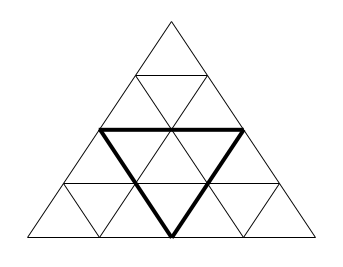
\includegraphics{triangle.png}
\end{center}

Напишите программу, которая будет определять, сколько всего в ней треугольников (необходимо учитывать не только "маленькие" треугольники, а вообще все треугольники — в частности, треугольник, выделенный жирным, а также вся фигура, являются интересующими нас треугольниками).

\InputFile

Вводится одно число N — количество уровней в фигуре ($1 \le N \le 100000$).  

\OutputFile

Выведите  количество треугольников в такой фигуре.

\Examples

\begin{example}
\exmp{
1
}{%
1
}%
\exmp{
2
}{%
5
}%
\exmp{
4
}{%
27
}%
\end{example}
\end{problem}
